\selectlanguage{Brazilian}

\chapter{MATERIAIS E MÉTODOS}\label{cap3}

\section{Modelagem Cinemática da Mão}

\subsection{Cinemática Direta da Mão}
\label{cinematica_direta_mao}
A partir do conjunto de restrições apresentado em \ref{anatomia_mao}, passamos a ter um modelo com 15 GL \cite{lin2000modeling}. E pode-se obter a cinemática direta, com o objetivo de calcular a posição e orientação da ponta do dedo a partir dos ângulos das juntas. A cinemática da mão pode ser subdividida em dois conjuntos: cinemática do polegar e cinemática dos dedos restantes. A cinemática direta é obtida por meio das matrizes de parâmetros de Denavit-Hartenberg (DH) \cite{hartenberg1964kinematic}, estas são frequentemente utilizadas em modelagem de braços robóticos \cite{cobos2008efficient}.

A transformação de Denavit-Hartenberg é a mais utilizada para representação cinemática de juntas concatenadas. Ela é baseada na transformação entre juntas sucessivas, e estas expressas por 3 parâmetros fixos e um variável (dependente do tipo de junta) \cite{newman2000calibration}. Os parâmetros de DH que, portanto, descrevem as juntas são: $a_i$, que representa o comprimento da conexão entre duas juntas; $\alpha_i$, que representa a rotação entre uma junta e o sua sucessiva dado o eixo de ação da junta; $d_i$, que representa \textit{offset} da junta, ou seja, a distância de uma junta até a próxima ao longo do eixo de ação de i; e $\theta_i$, que representa o ângulo de uma junta, ou seja, a rotação de uma junta em relação a próxima sobre o eixo de ação de i. Os parâmetros $a_i$ e $\alpha_i$ são os parâmetros que definem a posição relativa de duas juntas no espaço, enquanto os parâmetros $d_i$ e $\theta_i$ são os parâmetros variáveis, que definem o tipo da junta\cite{corke2007simple}.

A representação de DH é feita, portanto, por matrizes de transformação, as quais relacionam as coordenadas de uma junta i em relação a base do sistema por meio de:

\begin{align}
\label{RepDH}
A_i(\theta_i,d_i,a_i,\alpha_i) = R_z(\theta_i)T_z(d_i)T_x(a_i)R_x(\alpha_i)
\end{align}

Onde $R_k$ representa a rotação em torno do eixo \textit{k} e $T_k$ representa a translação ao longo do eixo \textit{k}. Para um manipulador com n juntas pode-se expressar a transformação total do manipulador em função das transformações de suas juntas individuais \cite{corke2007simple}.

\begin{align}
\label{TransDH}
T^{0}_n = A^{0}_1 A^{1}_2 ... A^{n-1}_n
\end{align}

\cite{craig2005introduction} expressou um conjunto de juntas genéricas para exemplificar o conceito da obtenção dos parâmetros de DH

\begin{figure}[H]
\centering
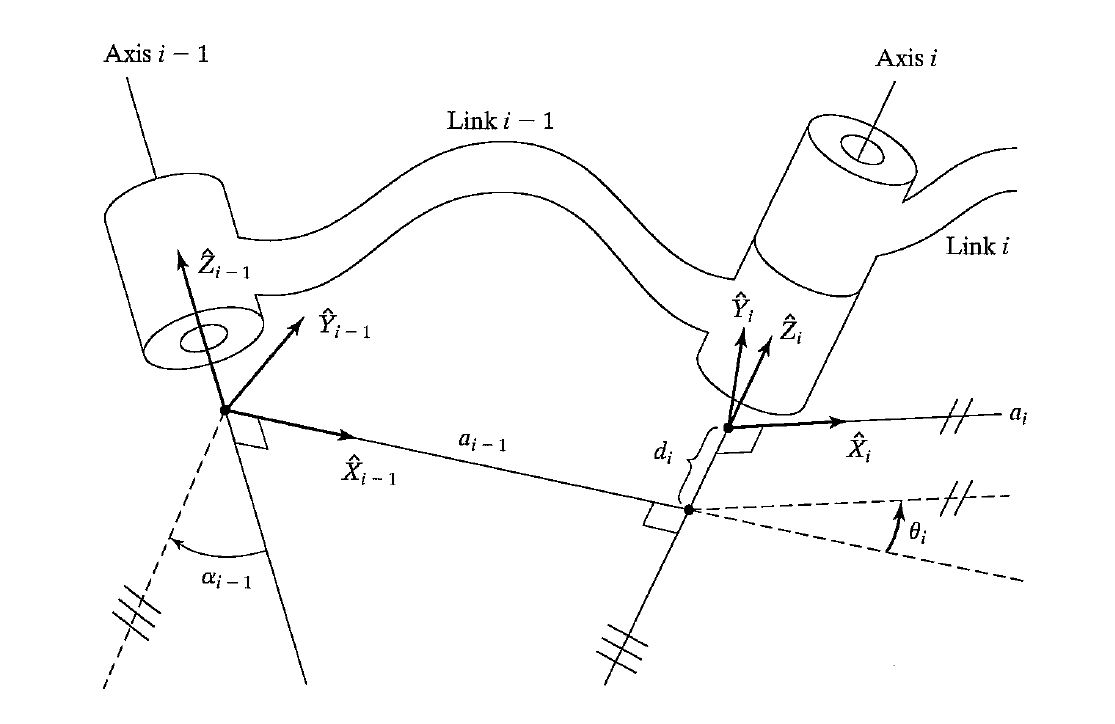
\includegraphics[width = 0.8\textwidth]{img/Craig_DHLinks.JPG}
\caption[Representação das Juntas para Obtenção dos Parâmetros de DH]{Juntas Genéricas para DH \cite{craig2005introduction}}
\label{Rocha2011}
\end{figure}

\subsubsection{Dedos Indicador, Médio, Anelar e Mínimo}
Sem considerar o osso metacarpo, que é o osso que faz a ligação dos dedos com a palma, os dedos indicador, médio, anelar e mínimo possuem 3 juntas: MP, PIP e DIP, e 3 ossos: próximo, médio e distal. Como definidas por \cite{lee1995model} as duas juntas flexivas mais a junta diretiva formam 4 GL. A tabela \ref{DHResto} mostra os parâmetros da matriz de DH e a figura \ref{JuntasResto} mostra a configuração das juntas para determinação dos parâmetros de DH.

\begin{table}[H]
\centering
\caption{Parâmetros da Matriz DH - Indicador,Médio,Anelar e Mínimo}
\label{DHResto}
\begin{tabular}{|c|c|c|c|c|}
	\hline
    Juntas & a & $\alpha$ & d & $\theta$ \\ \hline
    1 & 0 & $0^\circ$ & 0 & $\theta_1$ \\ \hline
    2 & 0 & $-90^\circ$ & 0 & $\theta_2$ \\ \hline
    3 & $l_1$ & $0^\circ$ & 0 & $\theta_3$ \\ \hline
    4 & $l_2$ & $0^\circ$ & 0 & $\theta_4$ \\ \hline
    5 & $l_3$ & $0^\circ$ & 0 & $\theta_5$ \\
	\hline
\end{tabular}
\end{table}

\begin{figure}[H]
\centering
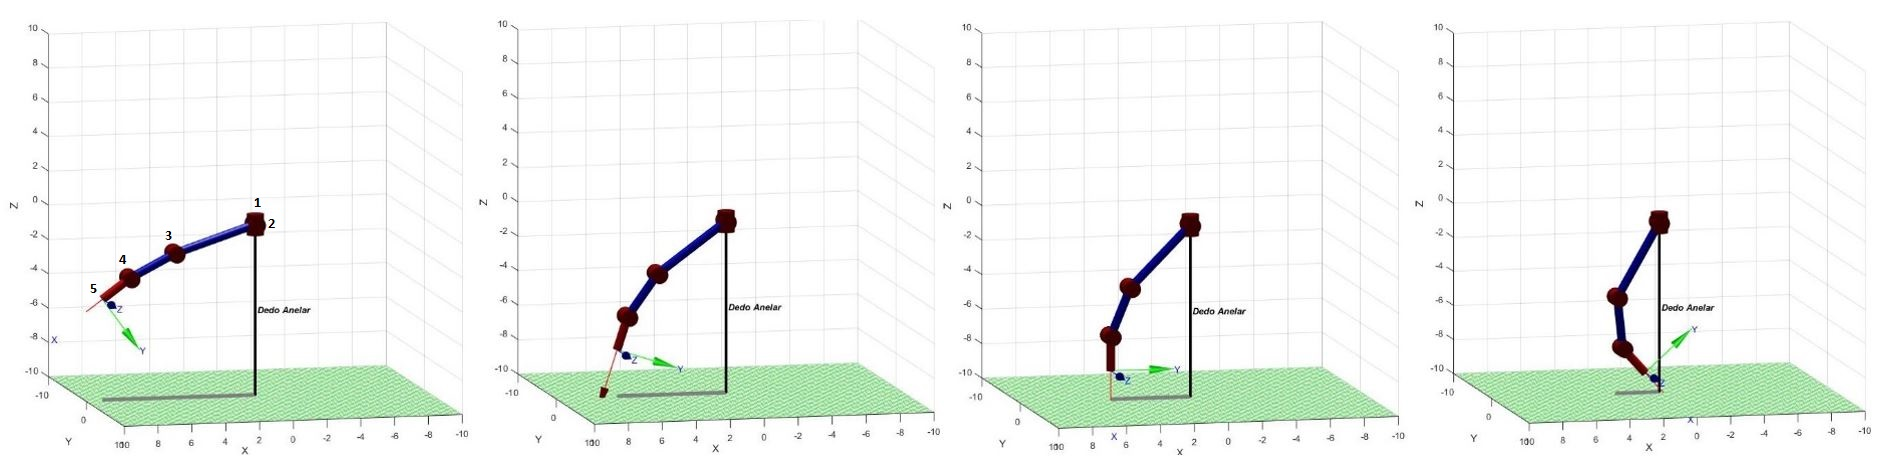
\includegraphics[width = 1\textwidth]{img/Anelar.JPG}
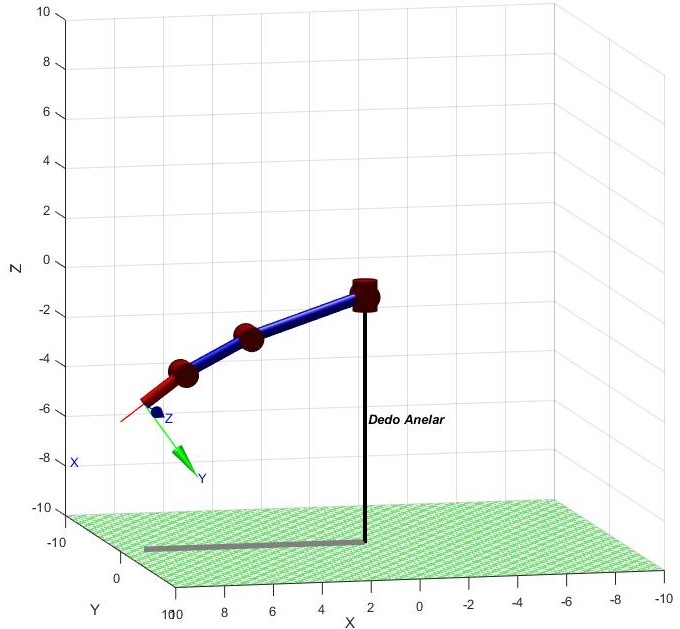
\includegraphics[width = 0.65\textwidth]{img/Anelar1.JPG}
\caption[Representação do dedo anelar como um manipulador robótico]{Representação do dedo anelar como um manipulador robótico utilizando o toolbox do \textit{MATLAB} \cite{corke1996robotics}}
\label{JuntasResto}
\end{figure}



\subsubsection{Dedo Polegar}
O polegar possui 3 juntas, sendo duas diretivas e uma flexiva, configurando 5 GL \cite{lee1995model}, e 3 ossos. A tabela \ref{DHPolegar} mostra os parâmetros da matriz de DH e a figura \ref{JuntasPolegar} mostra a configuração das juntas para determinação dos parâmetros de DH. A configuração para a construção do polegar prevê \textit{offsets} para as rotações de coordenadas das juntas, como na junta 4 e 5.

\begin{table}[H]
\centering
\caption{Parâmetros da Matriz DH - Polegar}
\label{DHPolegar}
\begin{tabular}{|c|c|c|c|c|}
	\hline
    Juntas & a & $\alpha$ & d & $\theta$ \\ \hline
    1 & 0 & $0^\circ$ & 0 & $\theta_1$ \\ \hline
    2 & 0 & $90^\circ$ & 0 & $\theta_2$ \\ \hline
    3 & 0 & $0^\circ$ & $l_1$ & $\theta_3$ \\ \hline
    4 & 0 & $90^\circ$ & 0 & $\theta_4 + \frac{\pi}{2}$  \\ \hline
    5 & -$l_2$ & $0^\circ$ & 0 & $\theta_5 - \frac{\pi}{2}$ \\ \hline
    6 & -$l_3$ & $0^\circ$ & 0 & $\theta_6$ \\
	\hline
\end{tabular}
\end{table}

\begin{figure}[H]
\centering
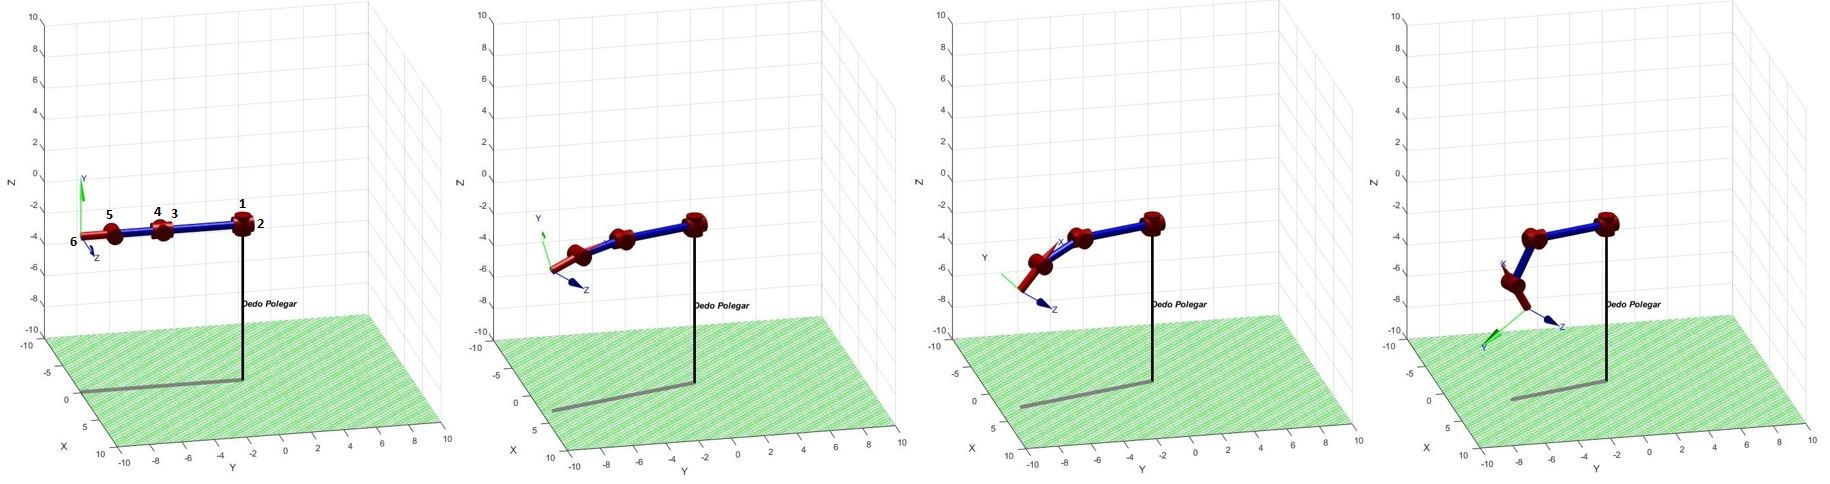
\includegraphics[width = 1\textwidth]{img/Polegar.JPG}
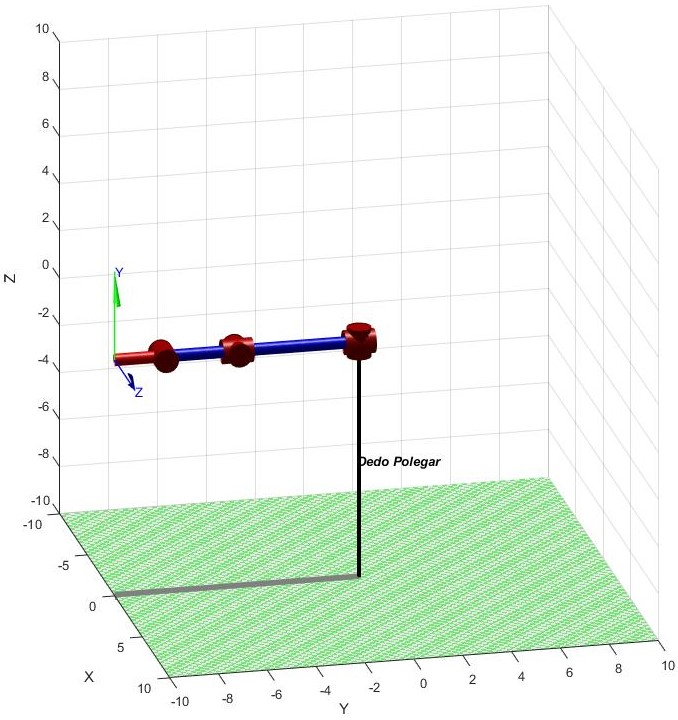
\includegraphics[width = 0.65\textwidth]{img/Polegar1.JPG}
\caption[Representação do dedo polegar como um manipulador robótico]{Representação do dedo polegar como um manipulador robótico utilizando o toolbox do \textit{MATLAB} \cite{corke1996robotics}}
\label{JuntasPolegar}
\end{figure}

\subsection{Simulação da Mão}
Neste projeto a simulação da mão é implementada utilizando uma toolbox do \textit{MATLAB} de código open source do proprietário Peter Corke \cite{corke1996robotics}, a "Robotics Toolbox for MATLAB". Com o uso desta toolbox é necessário implementar as matrizes de DH, que definirão os chamados \textit{Links} e ao unir-los, criando um \textit{SerialLink}, podemos definir as posições espaciais dos dedos utilizando a cinemática direta, ou seja, passando como parâmetros os ângulos de cada junta. Os ângulos de cada junta por sua vez são obtidos do modelo de Hill \cite{hill1938heat} que estão explicados com mais detalhes na seção \ref{modelagem_antebraco}. 

É possível criar uma visão de alto nível de como a modelagem cinemática da mão, e assim sua simulação, interage diretamente com a modelagem dos músculos do antebraço, e portanto o modelo de Hill, como na imagem \ref{IntegracaoAltoNivel}

\begin{figure}[H]
\centering
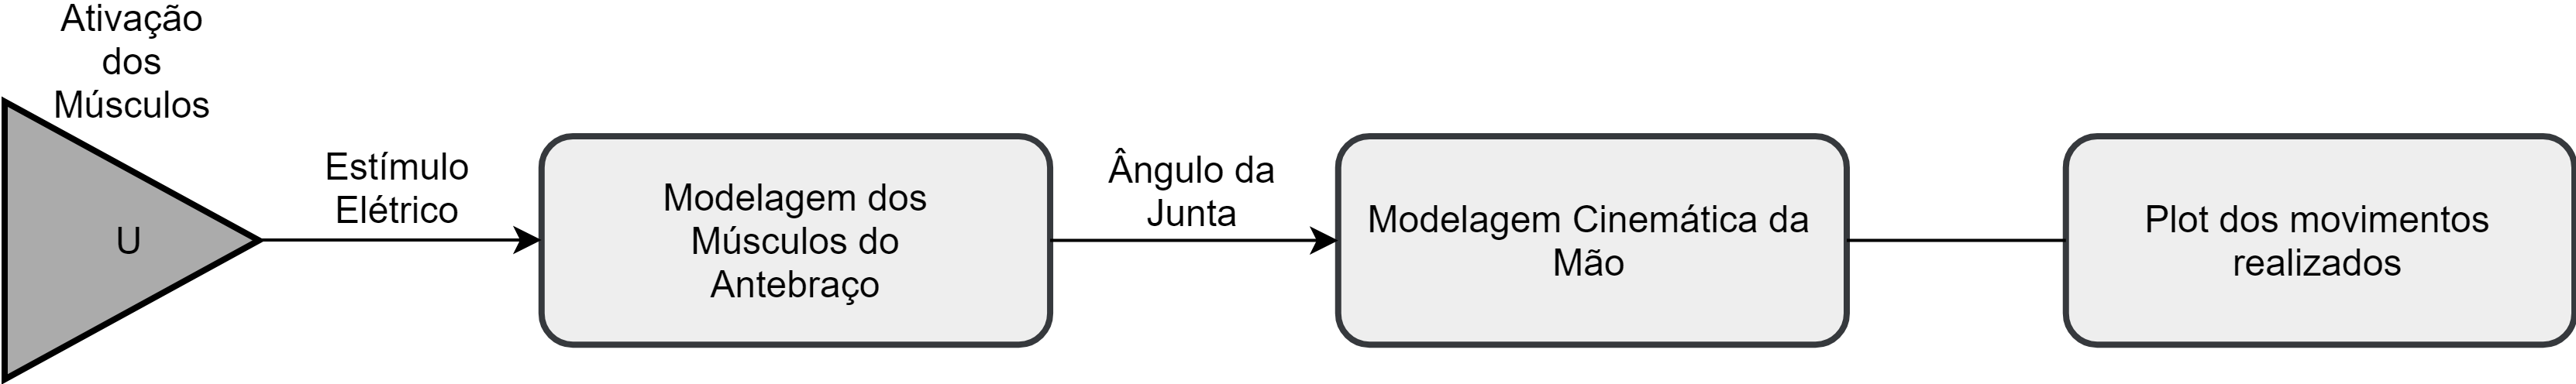
\includegraphics[width = 1\textwidth]{img/integracao_alto_nivel.JPG}
\caption[Integração em alto nível]{Integração em alto nível da modelagem cinemática da mão e da modelagem dos músculos do antebraço}
\label{IntegracaoAltoNivel}
\end{figure}

A implementação dos dedos neste projeto é, como apresentado na cinemática da mão, separada na cinemática do polegar e a cinemática dos demais dedos da mão.Para isto são utilizadas as matrizes de DH obtidas na seção \ref{cinematica_direta_mao}. Os referenciais do plano cartesiano são como os mostrados nas imagens \ref{JuntasResto} e \ref{JuntasPolegar}, tomando como base referencial a primeira junta, a que está na base da falange. Como é um modelo tridimensional, os ângulos das juntas permitem, com base nas restrições da seção \ref{anatomia_mao} descrever a posição dos dedos no espaço.

Dentre os parâmetros de DH, estão os parâmetros dados pela letra l que são, basicamente, as distâncias entre as juntas, e os parâmetros $\theta$ que definem a angulação da junta. Logo, para cada separação podemos definir de antemão os parâmetros estáticos (l) com base em medições realizadas sobre seres humanos comuns.

\begin{table}[H]
\centering
\caption{Parâmetros Definidos Para Indicador,Médio,Anelar e Mínimo}
\label{ParamResto}
\begin{tabular}{|c|c|c|c|c|}
	\hline
    Parâmetro & Valor (cm) & Observação \\ \hline
    $l_1$ & 3 & Comprimento Primeira Falange \\ \hline
    $l_2$ & 2,5 & Comprimento Segunda Falange \\ \hline
    $l_3$ & 2 & Comprimento Terceira Falange \\ \hline
\end{tabular}
\end{table}

\begin{table}[H]
\centering
\caption{Parâmetros Definidos Para o Polegar}
\label{ParamPolegar}
\begin{tabular}{|c|c|c|c|c|}
	\hline
    Parâmetro & Valor (cm) & Observação \\ \hline
    $l_1$ & 5,7 & Comprimento Primeira Falange \\ \hline
    $l_2$ & 4,2 & Comprimento Segunda Falange \\ \hline
    $l_3$ & 2,7 & Comprimento Terceira Falange \\ \hline
\end{tabular}
\end{table}

Uma vez utilizados os parâmetros definidos, é possível utilizando as matrizes de DH obter a posição espacial da ponta de cada dedo, com valores específicos em x,y e z para cada junta também.

\section{Modelagem dos Músculos do Antebraço}
\label{modelagem_antebraco}
Para simular o comportamento dos dedos, como descrito na imagem \ref{IntegracaoAltoNivel}, é necessário que sejam determinados os ângulos das juntas. Estes ângulos são determinados a partir da força produzida pelos músculos como é descrito no modelo de Hill na seção \ref{propriedades_musculo}. Para este projeto usa-se um modelo mais simplificado da relação $flv$ do que as relações descritas por \cite{rosen1999performances}, este modelo aproxima-se mais do modelo descrito por \cite{zajac1989muscle} e \cite{durfee1994estimation} em que o elemento SE pode ser desconsiderado assumindo ser infinitamente rígido, para fins de simplificação, já que a maior parte da força é gerada nos elementos CE e PE. Ao definir as curvas utilizadas no modelo podemos fazer de forma normalizada para que as variações nas medidas possam ser consideradas como ganhos simples.Para que haja adequação dos valores foram utilizados parâmetros encontrados em \cite{lemay1996dynamic}, os quais serão utilizados para determinar os valores dos ângulos das juntas.

\subsection{Músculos Utilizados}
É preciso determinar quais músculos serão tratados no problema, sabendo que cada músculo é responsável pelo movimento de uma, ou mais falanges. A partir da cinemática da mão proposta neste projeto 3 falanges serão movimentadas, as falanges próximas, as falanges médias e as falanges distais, sendo cada uma delas atrelada a uma junta, MP, PIP e DIP. Como simplificação do projeto é modelado que o movimento de avanço e recuo é realizado por músculos diferentes, apesar de agirem sobre a mesma falange e junta. 

Como descrito na restrição tipo 2 da seção \ref{anatomia_mao} a movimentação da falange distal é atrelada a movimentação da falange média, sendo definida pelo ângulo das juntas DIP e PIP. Logo são necessários 2 músculos para controlar os movimentos das juntas de flexão, e 4 músculos para os movimentos das juntas diretivas. Para efeitos de simplificação, o comprimento dos músculos de recuo tem o mesmo comprimento que os músculos de avanço, removendo assim a necessidade de se calcular mais parâmetros que não afetaram de forma expressiva a proposta deste projeto. Dada a imagem \ref{modelo_durfee} podemos notar que a força produzida por uma unidade muscular pode ser considerada de avanço ou recuo determinando o sinal de saída, logo podemos conectar ao modelo as forças dos músculos de avanço e recuo apenas alterando o sinal de saída de um tipo de músculo, aqui utilizaremos o sinal negativo para músculos de recuo.

\begin{figure}[H]
\centering
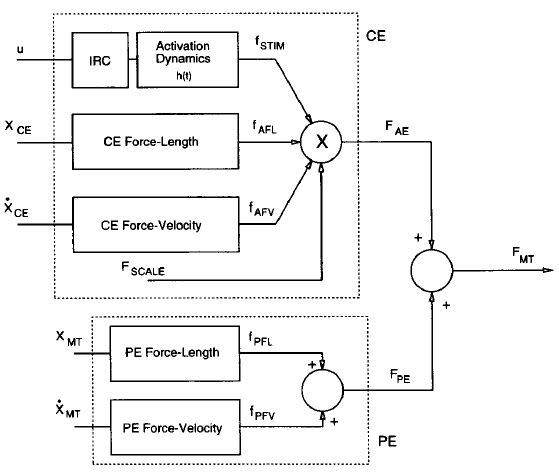
\includegraphics[width = 1\textwidth]{img/Durfee1994_Modelo.JPG}
\caption[Exemplo de Modelo Simplificado para Obter as Forças dos Músculos]{Modelo de um músculo eletricamente estimulado. A força proveniente do elemento CE é gerada por uma combinação multiplicativa de quatro fatores: ativação por estímulo, força-comprimento ativa, força-velocidade ativa e um fator de escala. A força proveniente do elemento PE é gerada por uma combinação somatória da força-comprimento passiva e da força-velocidade passiva 
\cite{durfee1994estimation}}
\label{modelo_durfee}
\end{figure}


\subsection{Forças de um Músculo a Partir de um Modelo Simplificado}
Como definido anteriormente, um modelo mais simplificado para se calcular a força líquida produzida por uma unidade motora pode ser descrito como em \cite{zajac1989muscle} onde a força é um resultado das propriedades força-comprimento e da força-velocidade, que estão dentro da dinâmica de contração. Em nosso modelo a entrada será a ativação dos elementos contráteis e a saída será a força produzida pela unidade motora, que pode ser extrapolada para um músculo inteiro.

O trabalho de \cite{zajac1989muscle} apresenta gráficos que definem o comportamento da força muscular $F^M$ em relação ao comprimento $l$ e a velocidade em que o músculo se deforma $v_m$. 

Os gráficos A e B definem uma propriedade estática do músculo e eles podem ser estudados quando o comprimento $L^M$ do músculo e o nível de ativação $a(t)$ são constantes. Uma ativação igual a 1 é considerada máxima quando os elementos contráteis do músculo forem excitados de forma máxima por muito tempo, ou seja, sem considerar mais o período transiente. Contrariamente um músculo é definido em repouso quando seu nível de ativação é 0, ou seja, inativo por muito tempo. A força identificada nos gráficos A e B é nomeada de força muscular ativa e esta força é gerada (nominalmente) entre $0,5{L_o}^M < L^M < 1,5{L_o}^M$, sendo ${L_o}^M$ o comprimento onde a força tem um pico (${F_o}^M$) \cite{zajac1989muscle}. Uma comparação entre os gráficos A e B mostra que músculos parcialmente ativados preservam as mesmas características que os músculos totalmente ativados.

Os gráficos C e D definem a propriedade da força-velocidade nos músculos. Quando um músculo é exposto a ativação máxima, ele fica sujeito a uma tensão constante, diminui e então para. O comprimento em que o músculo para então determina o comprimento no qual o músculo aguenta tal tensão no estado estático sob ativação máxima. Então os gráficos C e D podem ser utilizados para qualquer $L^M$ onde $0,5{L_o}^M < L^M < 1,5{L_o}^M$ \cite{zajac1989muscle}. Podemos retirar destes gráficos, então, qual a força $F^M$ que será exercida pelo músculo 

\begin{figure}[H]
\centering
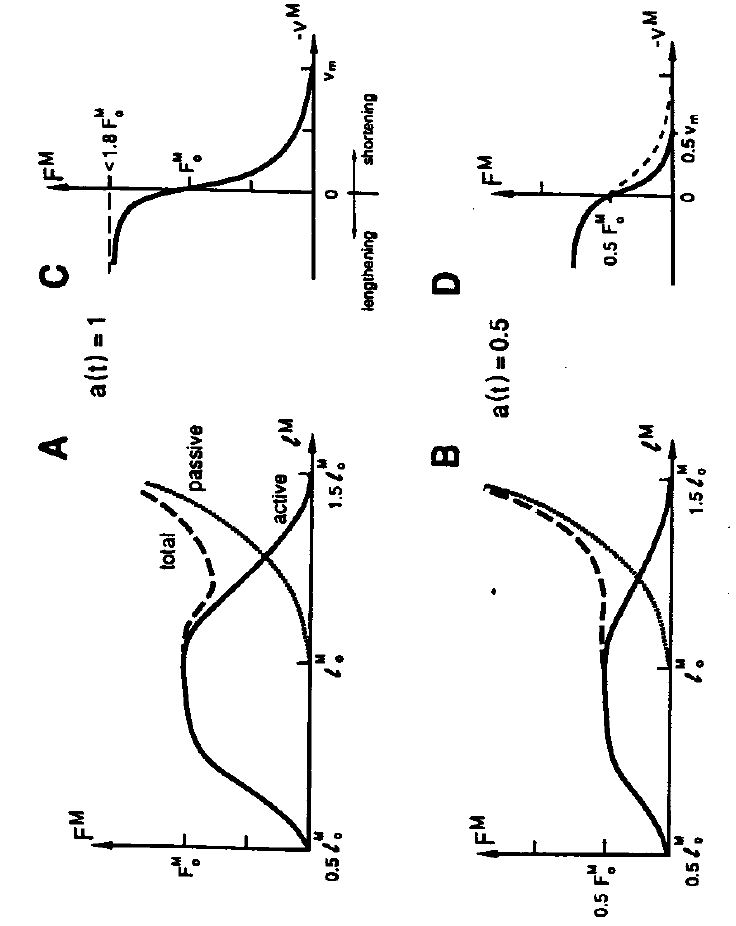
\includegraphics[width = 0.75\textwidth,angle=-90]{img/Zajac1989_Graficos.JPG}
\caption[Gráficos das propriedades força-comprimento e força-velocidade]{Propriedades do material dos tecidos musculares. (A e B) Propriedades estáticas
dos componentes passivo (PE) e ativo (CE) do músculo são dados através das curvas
normalizadas. $F^M$ e $L^M$ representam a força e o comprimento exercidos normalizados pelo
pico de força e pelo comprimento do músculo, respectivamente. (C e D) Propriedades
dinâmicas do músculo, do componente CE, é dada por uma relação adimensional entre
a força máxima que pode ser exercida e a velocidade do músculo. Note que $v_m$ também
é normalizado pelo máximo valor de $v_m$ do músculo. A amplitude das curvas C e D são
proporcionais ao nível de atuação (a), na curva C temos a = 1, na curva D temos a =
0,5.
\cite{zajac1989muscle}}
\label{graficos_zajac}
\end{figure}

As equações \ref{forcaCE} e \ref{forcaPE} no modelo de Hill demonstram as mesmas propriedades que as mostradas no gráfico \ref{graficos_zajac}. A força produzida pelo elemento PE depende somente do comprimento do músculo, enquanto a força produzida pelo elemento CE depende da $F_max$, do nivel de ativação a (ou $U$ na equação), e das propriedades força-comprimento e força-velocidade. Sendo assim é possível relacionar esses gráficos com aquelas equações estabelecidas anteriormente, sabendo que aqui pode-se determinar $F_max$ utilizando os gráficos C e D, que utilizam o nível de ativação e a velocidade com que o músculo se deforma. Portanto a curva estática do elemento ativo CE tem a amplitude modulada pela relação entre a ativação e a velocidade dada pela curva C, enquanto a curva estática do elemento passivo PE só depende do comprimento do músculo e tem um perfil exponencial.

Uma vez que o projeto será trabalhado no \textit{SIMULINK}, identificou-se uma facilidade em implementar o modelo a partir de uma interpolação das curvas determinadas por \cite{zajac1989muscle}. O \textit{MATLAB} foi utilizado para determinar polinômios capazes de representar de forma desejada as curvas descritas, os polinômios encontrados estão descritos em \ref{#1}

\begin{align}
F_{CE} = -0,8606x^5 + 12,39x^4 - 38,49x^3 + 43,6x^2 - 17,51x + 1,88 \label{funcCE} \\
F_{PE} = 8,13x^4 - 19x^3 + 15,07x^2 - 4,493x +0,3338 \label{funcPE}
F^M = F_{CE} + F_{PE} \label{funcFM}
F_{max} = 0,06757x^7 - 0,04067x^6 - 0,5223x^5 + 0,2424x^4 + 1,387x^3 - 0,4223x^2 - 1,844x + 1,12 \label{funcFMax}
\end{align}
